%%%%%%%%%%%%%%%%%%%%%%%%%%%%%%%%%%%%%%%%%%%%%%%%%%%%%%%%%%%%%%%%%%%%%%%%%%%%%%
% Jan Kalina <xkalin03@stud.fit.vutbr.cz> 2013
%%%%%%%%%%%%%%%%%%%%%%%%%%%%%%%%%%%%%%%%%%%%%%%%%%%%%%%%%%%%%%%%%%%%%%%%%%%%%%

%%%%%%%%%%%%%%%%%%%%%%%%%%%%%%%%%%%%%%%%%%%%%%%%%%%%%%%%%%%%%%%%%%%%%%%%%%%%%%
\chapter{Úvod} \label{uplnyUvod}
%%%%%%%%%%%%%%%%%%%%%%%%%%%%%%%%%%%%%%%%%%%%%%%%%%%%%%%%%%%%%%%%%%%%%%%%%%%%%%

Je-li tématem jakékoli prezentace libovolný server, téměř vždy přijde dříve či později řeč na problematiku bezpečnosti.
Okolo bezpečnosti serverů obecně bylo zpracováno již mnoho prací.

Mezi prvními mechanismy, kterými se vynasnažíme server zabezpečit, bude pravděpodobně protipožární přepážka (Firewall), jež předejde útokům na služby poskytované serverem, jež nebyly určeny veřejnosti nebo koncovým zákazníkům.

Hned dalším opatřením, kterým se server budeme snažit zabezpečit, budou oprávnění operačního systému, ať již unixová, nebo např. SELinuxu. Tím můžeme znemožnit neoprávněný přístup jednoho softwarového serveru k datům jiného softwarového serveru.

Běží-li ale v rámci jednoho softwarového serveru aplikace různých provozovatelů, například jedná-li
se o poskytování webhostingu nebo hostování aplikací, žádný z těchto mechanismů nebude nic platný.

Firewall ani operační systém neoprávněnému přístupu jedné aplikace k datům jiné aplikace, v případě že obě běží v rámci jednoho počítače, v rámci jediného procesu a tedy i pod jediným uživatelským účtem, nemůže nijak zabránit.

Jednotlivé aplikace běžící v rámci jediného aplikačního serveru je schopný rozlišit, kromě samotného aplikačního serveru, jen virtuální stroj Javy, běhové prostředí v němž aplikační server běží.

Na úrovni virtuálního stroje Javy je tak možné vyladit oprávnění jednotlivých aplikací a součástí aplikačního serveru mimořádně jemně, za pomoci tzv. bezpečnostních politik.

Pohybujeme-li se ale v prostředí velkých poskytovatelů hostovaných aplikací, jediný server leckterým aplikacím
mnohdy nestačí a požadavky kladené na aplikaci jsou rozprostírány mezi celé skupiny aplikačních serverů.

Právě v tu chvíli se objevuje potřeba spravovat bezpečnostní politiky nasazené na jednotlivých serverech centrálně, napříč tímto distribuovaným prostředím.

Právě cetralizací správy bezpečnostních politik v Javě se proto zabývá tato práce.

Systém pro centralizovanou distribuci a výměnu bezpečnostních politik byl implementován jako rozšíření aplikačního serveru
WildFly a webové uživatelské rozhraní bylo vytvořeno jako rozšíření administrační webové konzole WildFly, HAL.

Práce je členěna do 7 kapitol, z nichž 1. je úvod, 2. -- 3. představuje informace potřebné pro implementaci práci tohoto zaměření,
4. a 5. popisuje samotnou implementaci systému, 6. kapitola popisuje jeho testování a výsledky práce jsou shrnuty v Závěru.

%%%%%%%%%%%%%%%%%%%%%%%%%%%%%%%%%%%%%%%%%%%%%%%%%%%%%%%%%%%%%%%%%%%%%%%%%%%%%%
\chapter{Bezpečnost v Javě} \label{teoretickyUvod}
%%%%%%%%%%%%%%%%%%%%%%%%%%%%%%%%%%%%%%%%%%%%%%%%%%%%%%%%%%%%%%%%%%%%%%%%%%%%%%

%=============================================================================
\section{Bezpečnost}
%=============================================================================

Protože se tato práce zabývá bezpečností, což je pojem, který lze v různých souvislostech chápat zcela odlišně, je nanejvýš vhodné nejprve specifikovat co termínem bezpečnosti míníme a z kterého pohledu se jí budeme zabývat.

Scott Oaks definuje ve své knize Java Security bezpečnost jako souhrn následujících kritérií: \cite[1.1]{oaks}

\begin{itemize}
  \item {\bf Bezpečí vůči zákeřnému software} -- programy by neměly být schopny poškodit prostředí hostitelského počítače.
  \item {\bf Bezpečí vůči Velkému bratru} -- programům by mělo být bráněno ve sledování uživatele -- programy by neměly být schopny svévolně číst soukromé informace na počítači, na kterém běží, ani na síti, ke které je tento počítač připojen.
  \item {\bf Autentizace} -- identita autorů programu by měla být ověřována (typicky pomocí digitálního podpisu).
  \item Šifrování -- data odesílaná a přijímaná programem by měla být šifrována.
  \item Auditovatelnost -- potenciálně škodlivé operace by měly být vždy zaznamenávány.
  \item Specifikovanost -- program by měla doprovázet specifikace bezpečnostních pravidel, které program dodržuje.
  \item Verifikovanost -- pro prováděné operace by měla být stanovena pravidla, proti kterým by měly být verifikovány.
  \item Dbaní na dobré vychování -- programům by mělo být bráněno v užívání příliš mnoha systémových prostředků.
\end{itemize}

V souvislosti s víceuživatelskými prostředími se pak pojem bezpečnosti vyskytuje ještě v další rovině, kdy nejde o bezpečí systému před běžící aplikací, ale o způsob jakým může naopak program ověřit, kdo je jeho uživatelem a zdali má právo po něm žádat vykonání operace, o jejíž vykonání žádá.

Tato práce se zabývá bezpečností ve smyslu prvních tří bodů uvedeného výčtu (zvýrazněny tučně). Bude se tedy zabývat způsobem ochrany prostředí hostitelského počítače před jeho poškozením nebo neoprávněným sledováním ze strany běžících programů. Právě oprávnění programu pak souvisí s autentizací. Autentizací se myslí ověřování autorství programu. Právě od toho, kdo je autorem programu, se totiž mohou oprávnění programu odvozovat.

%=============================================================================
\section{Java}
%=============================================================================

Programy v jazyce Java bývají překládány do platformě nezávislého a efektivněji než kód v jazyce Java interpretovatelného mezikódu, takzvaného bajtkódu.
Bajtkód ({\tt Bytecode}) bývá zpravidla interpretován virtuálním strojem Javy (JVM - Java Virtual Machine).

JVM je abstraktní výpočetní stroj. Podobně jako reálné výpočetní stroje má svoji instrukční sadu a paměť, se kterou může manipulovat, ale na rozdíl od nich pro něj neexistuje jeho fyzická implementace, pouze emulovaná implementace softwarová.

To znamená že její kód není prováděn nativně hardwarem, ale je interpretován speciálním programem, interpretem, který je sám zkompilován do nativního kódu dané platformy a prováděn jejím hardwarem.
To mimo nezávislosti na platformě přináší také vyšší stupeň abstrakce.

Díky tomu, že programy nepřistupují ani nemohou přistupovat ke zdrojům fyzického stroje přímo, ale pouze zprostředkovaně skrze zdroje virtuální stroje Javy, si není těžké představit, že by použití takovéhoto virtuálního stroje mohlo mít i významný bezpečnostní efekt.
Protože programy v JVM mohou k fyzickým zdrojům počítače (např. k souborům nebo k síti) přistupovat jen skrze JVM, zablokování takového přístupu ze strany JVM není nikterak složité - JVM stačí odmítnout takový požadavek a interpretovaný program nemá možnost JVM obejít.

%=============================================================================
\section{Správce bezpečnosti v Javě} \label{securityManager}
%=============================================================================

Pro maximální nastavitelnost omezení kladených na programy běžících na virtuálních strojích Javy nerozhoduje o povolení nebo zablokování operace nad zdrojem JVM samotná JVM, ale dotazuje se speciálního objektu -- tzv. správce bezpečnosti.

Správce bezpečnosti je instancí třídy {\tt java.lang.SecurityManager}, nebo její podtřídy. Podtřída je třída dědící atributy a metody (operace, přijímané zprávy) třídy, které je podtřídou.

Jakákoli podtřída třídy {\tt SecurityManager} tedy bude vždy přijímat všechny zprávy, které přijímá třída {\tt SecurityManager}, přičemž ty, které nebude sama implementovat, budou přejaty z její nadtřídy {\tt SecurityManager}.

Reference na instanci podtřídy může být vložena do proměnné určené pro referenci na instanci její nadtřídy.

Třídu jejíž instanci JVM použije při svém startu jako objekt správce bezpečnosti lze ovlivnit skrze konfigurační proměnnou JVM {\tt java.security.manager}.

Aplikace může referenci na aktuálně používaný správce bezpečnosti získat voláním {\tt System.getSecurityManager() } a vypnout nebo vyměnit voláním {\tt System.setSecurityManager()}. Volání těchto metod je samo chráněno správcem bezpečnosti. Nehrozí tedy, že by se program neoprávněně zbavil omezení, která na něj správce bezpečnosti uvalil, jeho vypnutím nebo výměnou.

Hodnotu konfigurační proměnné {\tt java.security.manager} je při startu JVM možné nastavit za pomoci k tomu určeného parametru {\tt -D}. Pro spuštění programu s výchozím správcem bezpečnosti můžeme tedy použít příkaz:

\begin{lstlisting}[caption=Příkaz spouštějící program s výchozím správcem bezpečnosti, label=smEx]
java -Djava.security.manager=default ProgramABC
\end{lstlisting}

Příklady možných hodnot proměnné {\tt java.security.manager} a jim odpovídající třídy objektů správce bezpečnosti popisuje tabulka \ref{tabulkaParametruJavy}.

\begin{table}[tb]
\label{tabulkaParametruJavy}
\begin{center}
    \begin{tabular}{| l | l |}
    \hline
    Parametr příkazu {\tt java}                              & {\tt System.getSecurityManager()} \\ \hline
    (parametr nepoužit)                                      & {\tt null                       } \\
    {\tt -Djava.security.manager                           } & {\tt java.lang.SecurityManager  } \\
    {\tt -Djava.security.manager=default                   } & {\tt java.lang.SecurityManager  } \\
    {\tt -Djava.security.manager=java.lang.SecurityManager } & {\tt java.lang.SecurityManager  } \\
    {\tt -Djava.security.manager=TestovaciSM               } & {\tt TestovaciSM                } \\
    \hline
    \end{tabular}
\end{center}
\caption{Příklady možných hodnot proměnné {\tt java.security.manager}}
\end{table}

Správce bezpečnosti není použit jen v případě, že konfigurační proměnná {\tt java.security.manager} není vůbec definována, k čemuž běžně stačí nepoužít uvedeného parametru. Pokusí-li se aplikace získat referenci na používaného správce bezpečnosti, bude jí vrácena hodnota {\tt null}, jak ukazuje 1. řádek tabulky.

Bude-li tato konfigurační proměnná definována jako prázdná nebo obsahující řetězec {\tt default}, bude jako objekt správce bezpečnosti použita nová instance výchozí třídy správce bezpečnosti -- {\tt java.lang.SecurityManager}. To je naznačeno 2. a 3. řádkem tabulky.

V případě jiného obsahu této konfigurační proměnné bude jako objekt správce bezpečnosti použita nová instance třídy určené názvem z hodnoty této konfigurační proměnné, jak je nazvačeno posledním řádkem tabulky.

Poslední řádek tabulky zároveň demonstruje způsob použití objektu vlastní třídy správce bezpečnosti. Způsob vytvoření vlastní třídy správce bezpečnosti bude podrobněji rozebrán v kapitole \ref{vlastniSM}. Jestliže je zde uvedena neexistující třída, skončí inicializace JVM výjimkou a vykonávání programu nebude vůbec zahájeno:

\begin{lstlisting}[caption=Vyjímka při spuštění JVM s neexistujícím správcem bezpečnosti, label=smEx]
Error occurred during initialization of VM
java.lang.InternalError: Could not create SecurityManager: neexistujici.SM
    at sun.misc.Launcher.<init>(Launcher.java:106)
    at sun.misc.Launcher.<clinit>(Launcher.java:57)
    at java.lang.ClassLoader.initSystemClassLoader(ClassLoader.java:1486)
    at java.lang.ClassLoader.getSystemClassLoader(ClassLoader.java:1468)
\end{lstlisting}

Tím, že je zabráněno startu JVM v případě chybné konfigurace správce bezpečnosti, je tedy uplatněn bezpečnostní princip, kdy systém zůstane bezpečný i v případě poruchového stavu.

Z výpisu obsahu zásobníku volání můžeme vidět, že k vytvoření a použití objektu správce bezpečnosti dochází v rámci kontruktoru třídy {\tt sun.misc.Launcher}. Její instance je vytvářena v rámci inicializace systémového zavaděče tříd (System Class Loader), jež je prováděna při prvním pokusu o jeho získání. (Význam zavaděče tříd bude později rozebrán v kapitole \ref{classloader}.)

%=============================================================================
\section{Implementace vlastního správce bezpečnosti} \label{vlastniSM}
%=============================================================================

V této podkapitole bude vysvětlen způsob stanovení bezpečnostní politiky vytvořením vlastního správce bezpečnosti.
Správce bezpečnosti je objekt, na který JVM při požadavku na Java API deleguje rozhodnutí o povolení nebo nepovolení operace nad zdrojem.
Tento objekt musí být instancí třídy {\tt java.lang.SecurityManager} nebo její podtřídy. \cite{tutorialsTSM}

Algoritmus používaný Java API pro rozhodnutí o vykonání nebo nevykonání potenciálně nebezpečné operace je následující: \cite[4.1.1]{oaks}

\begin{enumerate}
  \item Uživatelská aplikace žádá prostřednictvím Java API o provedení dané operace
  \item Java API se dotáže správce bezpečnosti zda operaci povolit zavoláním patřičné metody správce bezpečnosti.
  \item Nemá-li být operace povolena, vrátí správce bezpečnosti výjimku {\tt SecurityException}, která je předána uživatelské aplikaci, čímž je vykonání operace zabráněno.
  \item Není-li vyhozena žádná výjimka, operace se považuje za povolenou a je provedena.
\end{enumerate}

Vlastního správce bezpečnosti tedy vytvoříme rozšířením třídy {\tt SecurityManager}, přičemž přepíšeme metody rozhodující o povolení akce, kterou chceme povolit, nebo pro kterou chceme stanovit vlastní algoritmus rozhodující zda akci povolit nebo ne.
Protože standardní správce bezpečnosti implicitně všechny operace zakazuje, stačí nám implementovat metody autorizující provedení operací, které chceme povolit a operacemi které nikdy povolit chtít nebudeme se nebudeme muset zabývat.

Příklad níže ukazuje jednoduchý správce bezpečnosti, který o povolení každé akce rozhodne na základě interakce s uživatelem. Při pokusu programu o provedení potenciálně nebezpečné operace je uživateli zobrazen dotaz, zda chce tuto operaci povolit nebo ne. V případě negativní odpovědi je jejímu provedení vrácením výjimky {\tt SecurityException} zabráněno.

\begin{lstlisting}[caption=Jednoduchý správce bezpečnosti, label=TestovaciSM]
public class TestovaciSM extends SecurityManager {
	@Override
	public void checkPermission(Permission permission) {
		
		System.out.println("Povolit " + permission.toString() + " ?");
		if(!askUser()){ // jestlize uzivatel nezvoli "povolit"
			throw new SecurityException("Operace byla zakazana uzivatelem");
		}
		
	}
}
\end{lstlisting}

V rámci vlastní aplikace je pak možné takto vytvořený správce bezpečnosti začít používat za pomoci dříve zmíněného příkazu:

\begin{lstlisting}[caption=Nastavení správce bezpečnosti zevnitř JVM, label=setSM]
System.setSecurityManager(new TestovaciSM());
\end{lstlisting}

Z vně aplikace je možné použití tohoto správce bezpečnosti nastavit při startu JVM vhodným nastavením konfigurační proměnné, jak je popsáno v kapitole \ref{securityManager}:

\begin{lstlisting}[caption=Spuštění aplikace se správcem bezpečnosti, label=runWithSM]
java -Djava.security.manager=TestovaciSM HelloWorld
\end{lstlisting}

Nutno dodat, že tato konfigurační proměnná je uplatněna pouze při startu JVM. Její změnou za běhu JVM nebude použití security manageru ovlivněno.

Zde uvedený správce bezpečnosti je opravdu pouze demonstrativní, v čemž se můžeme utvrdit, spustíme-li jej nad jednoduchou aplikací Hello world. Na správce bezpečnosti bude i v tomto jednoduchém případě kladeno celkem 29 dotazů.

Jelikož samotný výpis textu na standardní výstup není operací kontrolovanou správcem bezpečnosti, je příčinou všech dotazů na správce bezpečnosti inicializace samotného virtuálního stroje Javy.

V 18 případech je příčinou dotazu čtení obsahu konfiguračních proměnných (Property), v 8 případech jde o manipulaci s vlákny (Thread) a ve zbývajících 3 případech jde o čtení samotného souboru spouštěné třídy ({\tt Program.class})

Množství dotazů kladených na správce bezpečnosti je tedy i u takto primitivní aplikace příliš velký, než aby bylo možné nechat je zodpovídat uživatelem a vytvořit tak správce bezpečnosti pracujícího na principu interaktivní protipožární přepážky (firewall), nebyl by-li zároveň vytvořen předdefinový seznam vždy povolených operací.

Stanovení bezpečnostní politiky vytvořením vlastního správce bezpečnosti ale nepochybně možné je. Vyžaduje ale znalosti programování v Javě od správce počítače, na němž JVM běží. Od Javy verze 2 se tedy vytvoření vlastního správce bezpečnosti pro stanovení bezpečnostní politiky nepoužívá.

%=============================================================================
\section{Zavaděče tříd} \label{classloader}
%=============================================================================

Než se dostaneme k v současnosti využívanému způsobu stanovování bezpečnostní politiky, pozastavíme se nad tématem zavádění tříd.
Ačkoli se na první pohled může zdát, že toto téma s bezpečností příliš nesouvisí, opak je pravdou.
Jen a pouze zavaděč tříd (Classloader), který třídu do paměti zavádí, totiž může určit původ třídy, od kterého se oprávnění kódu této třídy odvozuje.

Zavaděč je objekt odpovědný za načítání tříd a rozhraní v Javě. Na základně názvu třídy používaného v bajtkódu (např. {\tt java.lang.String} nebo {\tt java.security.KeyStore\$} {\tt Builder\$FileBuilder\$1}) se tuto třídu pokusí vyhledat a načíst do paměti. \cite{refClassLoader}

Třída každého zavaděče tříd musí být podtřídou třídy {\tt java.lang.ClassLoader} a musí implementovat metodu {\tt findClass()}. Ta je jádrem celého zavaděče -- provádí samotné vyhledání třídy podle názvu. Jejím výstupem je pak objekt třídy {\tt java.lang.Class} představující samotnou třídu. Při programování běžných aplikací můžeme na objekty této třídy narazit například při snaze získat název třídy neznámého objektu jako řetězec za běhu aplikace: \cite{refClassLoader}

\begin{lstlisting}[caption=Získávání názvu třídy neznámého objektu, label=getClassName]
Class classOfUnknown = unknown.getClass();
String nameOfClass = classOfUnknown.getName(); // "java.lang.String"
\end{lstlisting}

Každý objekt v Javě si totiž uchovává referenci na svoji třídu, představovanou již zmíněným objektem třídy {\tt Class}. Metody této třídy umožňují získávat různé informace o třídě, jako seznam atributů ({\tt java.lang.reflect.Field}), metod ({\tt java.lang.reflect.Method}), anotací ({\tt java.lang.annotation.Annotation}) nebo vnořených tříd, reprezentovaných opět objektem třídy {\tt Class}.

%-----------------------------------------------------------------------------
\subsection{Zdroje kódu a ochranné domény}
%-----------------------------------------------------------------------------

Zdroj kódu ({\tt java.security.CodeSource}) je souhrnem informací určujících původ třídy: \cite{sourceCodeSource}

\begin{itemize}
  \item {\tt location}: URL adresa, ze které byla třída načtena.
  \item {\tt signers} / {\tt certs}: Množina podepsaných autorů a množina jejich certifikátů. Tyto dvě informace jsou vzájemně odvoditelné. Pro vytvoření objektu Zdroje kódu tak postačuje jedna z nich a druhá z ní pak může být kdykoli odvozena.
\end{itemize}

Ochranná doména ({\tt java.security.ProtectionDomain}) je objektem spojujícím objekt třídy se zdrojem kódu a oprávněními. Konkrétně se skládá z následujících informací: \cite{sourceProtectionDomain}

\begin{itemize}
  \item {\tt codesource}: Zdroj kódu třídy reprezentovaný výše rozebranou třídou.
  \item {\tt classloader}: Zavaděč tříd, kterým byla ochranná doména přidělena.
  \item {\tt principals}: Role uživatele přihlášeného k programu.
  \item {\tt permissions}: Oprávnění kódu třídy.
\end{itemize}

Každá třída spadá vždy do jedné ochranné domény, která může být společná více třídám. Za nastavení ochranné domény i zdroje kódu odpovídá zavaděč třídy. Jen ten totiž může původ třídy s znát, protože jen on s jistotou ví, odkud byl její kód získán a jak a zdali byl podepsán.

%-----------------------------------------------------------------------------
\subsection{Interní zavaděč tříd} \label{interniZavadec}
%-----------------------------------------------------------------------------

Interní zavaděč tříd je zavaděč používaný pro načítání tříd samotného Java API a zavaděčů uživatelských tříd.
Je součástí JVM. Je napsán převážně v nativním kódu a k načítání tříd tedy využívá nativní metody pro přístup k souborovému systému operačního systému.
Interní zavaděč načítá třídy ze souborů, jejíž adresu odvozuje z názvu třídy, balíčku a proměnné prostředí {\tt CLASSPATH}. \cite[3.2.1]{oaks}

Je-li tedy JVM spuštěna následujícím příkazem:

\begin{lstlisting}[caption=Spuštění JVM s předefinovanou proměnnou {\tt CLASSPATH}, label=javaClasspath]
java -classpath /srv/classes muj.program.Test
\end{lstlisting}

Bude spuštěna třídní metoda {\tt main()} třídy {\tt Test}, jež bude hledána v souboru {\tt /srv/classes/muj/program/Test.class}.

O třídách načtených interním zavaděčem se často mluví jako o třídách bez zavaděče, protože jejich objekt {\tt Class} má referenci na zavaděč nastavenu na {\tt null}. \cite[3.2.1]{oaks} Zároveň je {\tt null}ová také ochranná doména takto načtených tříd. Třídy načtené interním zavaděčem tak nemají svá oprávnění omezena. \cite[5.4]{oaks}

Interní zavaděč je v současnosti používán k načítání jen nejzákladnějších tříd, zejména tříd Java API, tedy tříd používajících součásti napsané v nativním kódu. Ostatní třídy z {\tt CLASSPATH} jsou obvykle načítány Zavaděčem tříd z URL (viz. \ref{URLClassLoader}).

%-----------------------------------------------------------------------------
\subsection{Zavaděč tříd z URL} \label{URLClassLoader}
%-----------------------------------------------------------------------------

Zavaděč tříd z URL ({\tt URLClassLoader}) hledá třídy také na URL adresách určených polem objektů {\tt URL}, předaných jeho konstruktoru. Je jedním z nejpoužívanějších zavaděčů tříd v Javě -- používá se k vyhledávání méně základních tříd v umístěných určených proměnnou {\tt CLASSPATH}. Dokáže třídy načítat nejen z adresářů, ale i z JAR archivů je-li jako adresa uvedena adresa JAR archivu. \cite[3.2.5]{oaks}

\begin{lstlisting}[caption=Vytvoření vlastní instance zavaděče tříd z URL, label=urlclassloader]
URLClassLoader classLoader = new URLClassLoader(new URL[]{
    new URL("http://server/directory/"),
    new URL("file:/srv/classes/"),
    new URL("file:/srv/archive.jar")
}, parentClassloader);
Class myClass = classLoader.loadClass("my.package.MyClass");
\end{lstlisting}

Zavaděč tříd z URL je jedním z bezpečných zavaděčů ({\tt SecureClassLoader}). To znamená že automaticky nastavuje ochranou doménu třídám, které načítá.

Třídy pocházející ze stejného zdroje (s odpovídajícím {\tt CodeSource}) patří do stejné ochranné domény a mají tak stejná oprávnění. Navrácení vždy stejného objektu ochranné domény přitom zavaděč zajišťuje pomocí asociativního pole {\tt SecureClassLoader.pdcache}, jehož klíčem je objekt zdroje kódu a hodnotou objekt ochranné domény. \cite{sourceSecureClassLoader}

%=============================================================================
\section{Systém řízení přístupu a soubory bezpečnostní politiky}
%=============================================================================

Systém řízení přístupu ({\tt java.security.AccessController}) je mechanismus využívající ochranné domény tříd na zásobníku volání k rozhodnutí, zda operaci požadovanou programem povolit či nikoliv. 

Na oprávněnost volajícího kódu provést vybranou akci se jej může dotazovat uživatelský kód a veškeré rozhodování na něj zároveň deleguje standardní správce bezpečnosti v Javě verze 2 a novějších. \cite[5]{oaks}

Systém řízení přístupu tedy stejně jako správce bezpečnosti umožňuje omezit, zdali může být operace nad zdrojem provedena nebo ne. Zdroji zde však již nejsou jen zdroje samotné JVM, díky tomu že uživatelské procesy mohou systém řízení přístupu také využívat k omezení přístupu ke zdrojům, jež samy poskytují. \cite[5]{oaks}

Máme-li tedy například knihovní třídu zprostředkovávající přístup k databázi v souboru po záznamech, při použití oprávnění jen na úrovni Java API by bylo možné programu přidělovat oprávnění jen k celému souboru najednou. Jednotlivé záznamy databáze v souboru je možné považovat za samostatné zdroje a využít systém řízení přístupu k jejich ochraně.

Systém řízení přístupu je schopný pravidla bezpečnostní politiky načítat z textového konfiguračního souboru -- tzv. souboru bezpečnostní politiky. Vzniká tak mnohem snazší způsob stanovení bezpečnostní politiky, kterou budou programy v JVM omezeny -- namísto tvorby vlastní třídy správce bezpečnosti stačí pro stanovení bezpečnostní politiky poupravit textový soubor bezpečnostní politiky. \cite[5]{oaks}

Systém řízení přístupu rozhoduje o povolení nebo nepovolení operace na základně průniku oprávnění ochranných domén tříd metod, jež vedly k zavolání metody provádějící citlivou operaci. Na legálnost operace se systému řízení přístupu může dotazovat samotná volaná metoda (voláním metody {\tt checkPermission()}), nebo správce bezpečnosti na základě dotazu na legálnost operace od Java API.

%-----------------------------------------------------------------------------
\subsection{Implementace Systému řízení přístupu}\label{implementaceAC}
%-----------------------------------------------------------------------------

Systém řízení přístupu (Access Controller) je implementován třídou {\tt AccessController} a voláním jeho statických metod na něj standardní správce bezpečnosti deleguje rozhodnutí o legálnosti provedení potenciálně nežádoucí operace uživatelského programu. Konkrétně kontrolu obstarává metoda {\tt checkPermission(Permission)}, která v případě neoprávněnosti požadavku na provedení operace způsobí vyhození výjimky {\tt AccessControlException}. Jejím vstupem je objekt třídy {\tt Permission}, která reprezentuje oprávnění, jehož vlastnictví je testováno. \cite[5.5]{oaks}\cite[6]{oaks}

Následující příklad ukazuje způsob, jakým se může kód dotázat Systému řízení přístupu, zdali má zadané oprávnění: \cite[5.5]{oaks}

\begin{lstlisting}[caption=Příklad použití Systému řízení přístupu, label=pouzitiAC]
try {
    // ma tento program opravneni pripojit se na lokalni port 80?
    AccessController.checkPermission(
        new SocketPermission("localhost:80", "connect")
    );
    System.out.println("Pripojeni bylo povoleno");
} catch (AccessControlException ace) {
    System.out.println("Pripojeni bylo zamitnuto");
}
\end{lstlisting}

Systém řízení přístupu rozhoduje o povolení nebo nepovolení operace na základně průniku oprávnění ochranných domén tříd metod, jež vedly k zavolání metody {\tt checkPermission()}. Konkrétně jde o metody nacházející se během volání {\tt checkPermission()} na zásobníku volání (Stack trace). Volala-li tedy metoda {\tt main} třídy {\tt Main} metodu {\tt secured} třídy {\tt Secured}, která následně zavolala metodu {\tt checkPermission()}, musí mít požadované oprávnění přiděleny ochranné domény tříd {\tt Main} i {\tt Secured}, aby toto volání neskončilo výjimkou vyjadřující zamítnutí provedení operace ze strany Systému řízení přístupu. \cite[5.5]{oaks}\cite[6.1]{oaks}

%-----------------------------------------------------------------------------
\subsection{Privilegované bloky kódu}\label{privilegovaneBloky}
%-----------------------------------------------------------------------------

Vraťme se nyní k našemu příkladu, kdy chceme různým programům přidělovat oprávnění k jednotlivým databázovým záznamům jako k samostatným zdrojům systému, ale nechceme jim povolit přístup k samotnému databázovému souboru.

Ze způsobu fungování Systému řízení přístupu, tak jak jsme si jej zatím popsali, totiž vyplývá, že aby mohla knihovna zprostředkovávající přístup k databázi přistupovat k databázovému souboru, musí mít oprávnění pracovat s databázovým souborem jak samotná databázová knihovna, tak i každá třída podílející se na jejím volání.

Tento stav je samozřejmě nepřípustný, protože oprávnění na úrovni uživatelského kódu by tímto ztratila význam -- buď by k databázi nemohla přistupovat knihovna volaná kódem, jež má oprávnění jen k některým záznamům, nebo by naopak měl jakýkoli kód, který by potřeboval přistupovat k záznamům v databázi, oprávnění k celému databázovému souboru, čímž by mohl jakákoli omezení na úrovni knihovny zprostředkující přístup k databázi obejít.

Právě tento problém řeší privilegované bloky kódu. Kód v privilegovaném bloku je spuštěn se samostatným zásobníkem volání. Při ověřování oprávnění při přístupu k jakémukoli zdroji tak ověřování skončí u třídy s tímto blokem.

{\bf Část kódu knihovny, jež vložíme do privilegovaného bloku, bude tedy spuštěna s oprávněními této knihovny bez ohledu na oprávnění kódu, jež metodu knihovny zavolal.}

%,,,,,,,,,,,,,,,,,,,,,,,,,,,,,,,,,,,,,,,,,,,,,,,,,,,,,,,,,,,,,,,,,,,,,,,,,,,,,
\subsubsection{Příklad použití privilegovaného bloku}
%'''''''''''''''''''''''''''''''''''''''''''''''''''''''''''''''''''''''''''''

Tento příklad ukazuje jednoduchý příklad použití privilegovaného bloku: \cite{refAccessController}

\begin{lstlisting}[caption=Příklad použití privilegovaného bloku, label=prikladBloku]
class DatabazeVSouboru {
  public void provedOperaciNadDatabazi(){
    // Zde bude kod omezen opravnenimi volajici tridy
    AccessController.doPrivileged(new PrivilegedAction<Void>() {
      public Void run() {
        // Zde bude kod spusten nezavisle na opravnenich volajici tridy
      }
    }
  }
}
\end{lstlisting}

Vykonávání privilegovaného bloku je implementováno jako nativní metoda Systému řízení přístupu {\tt doPrivileged()}, které je předán objekt (pod)třídy {\tt PrivilegedAction}. Jeho metoda {\tt run()} je spuštěna privilegovaně, tedy bez ohledu na oprávnění tříd na zásobníku volání.

%,,,,,,,,,,,,,,,,,,,,,,,,,,,,,,,,,,,,,,,,,,,,,,,,,,,,,,,,,,,,,,,,,,,,,,,,,,,,,
\subsubsection{Příklad s knihovnou pro přístup k databázi}\label{databazeVsouboru}
%'''''''''''''''''''''''''''''''''''''''''''''''''''''''''''''''''''''''''''''

Tento příklad ukazuje možnou implementaci knihovny pro přístup k databázi, jak byla navržena v kapitole \ref{privilegovaneBloky}.

\begin{lstlisting}[caption=Demonstrační knihovna pro přístup k databázi, label=pouzitiAC]
class DatabazeVSouboru {
  public Zaznam nactiZaznam(String klic){
    
    // volajici kod musi mit opravneni k nacteni zaznamu
    AccessController.checkPermission(new ZaznamPermission(klic,"nacteni"));
    
    return AccessController.doPrivileged(new PrivilegedAction<Zaznam>() {
      public Zaznam run() {
        // provedeni operace nad samotnymi daty (s opravnenimi knihovny)
      }
    });
  }
}
\end{lstlisting}

Každá metoda knihovny zpřístupňující záznam v databázi nejprve ověří oprávněnost požadavku na přístup k danému záznamu. Tato kontrola se provede triviálně, stejně jako v příkladu \ref{pouzitiAC}.

Zde je důležité poznamenat že tato kontrola se musí provést mimo privilegovaný blok, čímž bude vlastnictví kontrolovaného oprávnění vyžadováno (mimo kódu samotné knihovny) také po kódu, jež tuto operaci nad záznamem volá. Pokud některá z tříd na zásobníku volání nebude mít požadované oprávnění, provádění operace nad databází bude přerušeno vyjímkou Systému řízení přístupu ({\tt java.security.AccessControlException}).

Jinak se pokračuje provedením samotné operace nad databází v rámci privilegovaného bloku. Tím bude tato operace provedena s oprávněními třídy knihovny, nezávisle na oprávněních kódu, jež metodu knihovny volal.

%-----------------------------------------------------------------------------
\subsection{Třídy oprávnění}
%-----------------------------------------------------------------------------

Třída oprávnění představuje typ zdroje, ke kterému lze přidělovat oprávnění.

Třída oprávnění musí být podtřídou třídy {\tt Permission}. Pro snazší implementaci je místo ní možné použít její podtřídu {\tt BasicPermission}.
Aby ji bylo možné použít, musí být definován její konstruktor odpovídající parametrům oprávnění předávaným souborem bezpečnostní politiky a musí být veřejně přístupná -- opatřená specifikátorem přístupu {\tt public}.

%,,,,,,,,,,,,,,,,,,,,,,,,,,,,,,,,,,,,,,,,,,,,,,,,,,,,,,,,,,,,,,,,,,,,,,,,,,,,,
\subsubsection{Příklad třídy oprávnění}
%'''''''''''''''''''''''''''''''''''''''''''''''''''''''''''''''''''''''''''''

Tento příklad ukazuje nejjednodušší způsob vytvoření vlastní třídy oprávnění na oprávnění použitém v příkladu s knihovnou pro přístup k databázi po záznamech v kapitole \ref{databazeVsouboru}.

\begin{lstlisting}[caption=Demonstrační třída oprávnění, label=prikladOpravneni]
public class ZaznamPermission extends java.security.BasicPermission {
    public ZaznamPermission(String name, String actions) {
        super(name, actions);
    }
}
\end{lstlisting}

%-----------------------------------------------------------------------------
\subsection{Soubory bezpečnostní politiky}
%-----------------------------------------------------------------------------

Tato kapitola popisuje implementaci bezpečnostních politik za pomoci souborů bezpečnostní politiky.

Soubor bezpečnostní politiky se skládá z deklarací původů tříd a jim přidělovaných oprávnění.
Původ třídy je zde stanoven na základě podpisu JAR archivu z kterého byla třída získána (direktiva {\tt signedBy}), URL kořene systému balíčků tříd (packages), ze kterého byla třída získána (direktiva {\tt codeBase}) nebo obou těchto kritérií najednou. \cite[5.3.1]{oaks}

Syntaxe souboru bezpečnostní politiky, používané standardní implementací bezpečnostní politiky {\tt PolicyFile}, je definována následovně: \cite[5.3.1]{oaks}

\begin{lstlisting}[caption=Syntaxe souboru bezpečnostní politiky, label=syntaxeSouboruBP]
grant [signedBy <autor>] [, codeBase <koren balicku>] {
    permission <trida opravneni> [<nazev zdroje> [, <povolovane operace>]];
    ...
};
\end{lstlisting}

Deklarace oprávnění se tedy skládá z názvu třídy oprávnění a parametrů jejího konstruktoru oddělených čárkou.

\begin{figure}[ht]
  \centering
  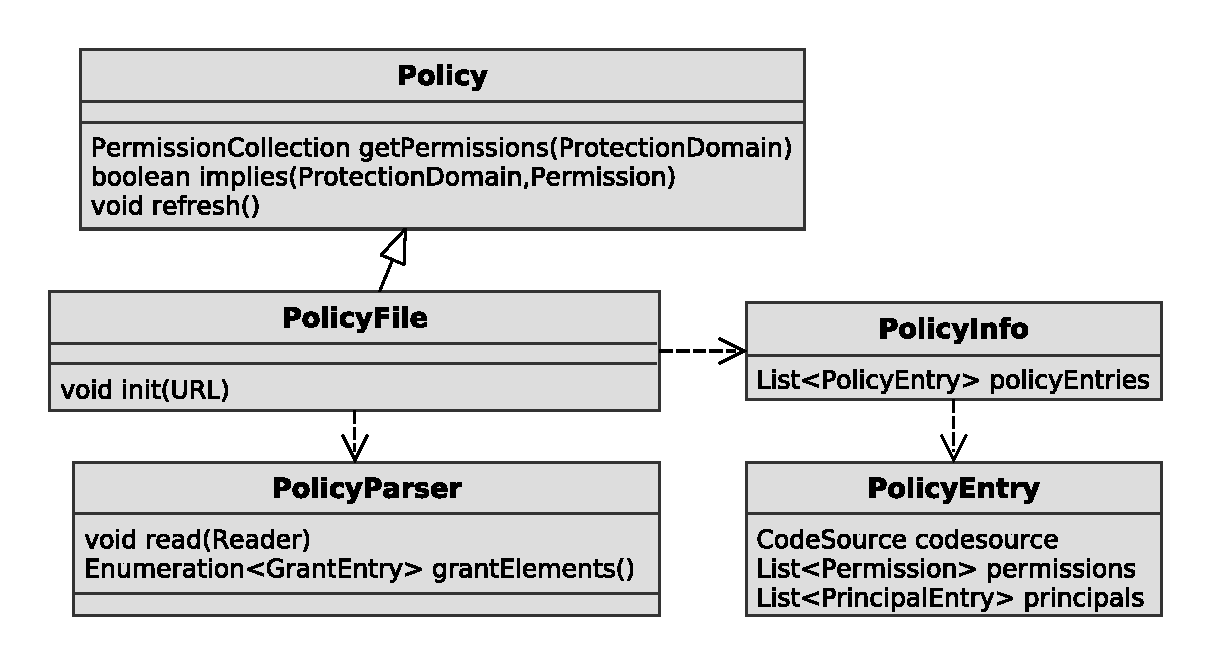
\includegraphics[width=14cm]{fig/policy-schema}
  \caption{Schéma tříd podílejících se na politice postavené na souboru politiky.}
\end{figure}

Standardní implementace bezpečnostní politiky {\tt PolicyFile} využívá {\tt PolicyParser} pro převod jednotlivých textových bloků {\tt grant} do objektové podoby.
Takto získaný výčet objektů {\tt GrantEntry} pak převádí na seznam objektů {\tt PolicyEntry}, které ukládá do atributu {\tt policyEntries} objektu vnitřní třídy {\tt PolicyFile.PolicyInfo}.

%,,,,,,,,,,,,,,,,,,,,,,,,,,,,,,,,,,,,,,,,,,,,,,,,,,,,,,,,,,,,,,,,,,,,,,,,,,,,,
\subsubsection{Příklad souboru bezpečnostní politiky}
%'''''''''''''''''''''''''''''''''''''''''''''''''''''''''''''''''''''''''''''

Tento příklad ukazuje jednoduchou bezpečnostní politiku, opět v kontextu příkladu knihovny pro přístup k databázi z kapitoly \ref{databazeVsouboru}.

\begin{lstlisting}[caption=Příklad souboru bezpečnostní politiky, label=prikladSouboruBP]
grant codeBase "file:/srv/program/" {
  permission ZaznamPermission "Lucka", "nacteni";
};
grant codeBase "file:/srv/knihovna/" {
  permission ZaznamPermission "*", "nacteni";
  permission java.io.FilePermission "/srv/knihovna/data/-","read,write";
};
\end{lstlisting}

Programu zde má přiděleno oprávnění k načtení záznamu \uv{Lucka}, nemůže ale přistupovat k s samotným databázovým souborů. K těm má oprávnění přistupovat jen knihovna zpřístupňující tuto databázi. Kvůli způsobu implementace kontroly oprávnění systémem řízení přístupu (popsaným v kapitole \ref{implementaceAC}) je nezbytné přidělit knihovně oprávnění ke všem záznamům v databázi, jinak by žádná kontrola oprávněnosti požadavku nemohla skončit pozitivně.

%,,,,,,,,,,,,,,,,,,,,,,,,,,,,,,,,,,,,,,,,,,,,,,,,,,,,,,,,,,,,,,,,,,,,,,,,,,,,,
\subsubsection{Zástupné znaky}
%'''''''''''''''''''''''''''''''''''''''''''''''''''''''''''''''''''''''''''''

URL kořene systému balíčků může být ukončeno zástupnými znaky pomlčka ({\tt -}) a hvězdička ({\tt *}).

Zatímco {\tt /*} odpovídá všem souborům v daném adresáři, {\tt /-} odpovídá všem souborům v daném adresáři i jeho podadresářích, rekurzivně. V obou případech jsou zahrnuty jak soubory tříd ({\tt .class}), tak i celé archivy tříd ({\tt .jar}/{\tt .war}/{\tt .ear}).
\cite{jdkdocPolicyFiles}

%-----------------------------------------------------------------------------
\subsection{Nastavení třídy a souboru bezpečnostní politiky}\label{souborPolitiky}
%-----------------------------------------------------------------------------

Nastavení třídy a souboru bezpečnostní politiky umožňuje správci nebo uživateli počítače stanovit bezpečnostní politiku aplikovanou na programy v Javě běžící na tomto počítači bez potřeby znalostí programování.

Obojí zmíněné je možné globálně, pro celé JRE, nastavit úpravou konfiguračního souboru {\tt java.security}, umístěného v podadresáři {\tt lib/security} adresáře JRE. \cite{refPolicyFiles}

Třída bezpečnostní politiky je určena svým celým jménem (např. {\tt sun.security.provider.PolicyFile}) a deklarována v konfigurační proměnné {\tt policy.provider}. \cite{refPolicyFiles}

Soubory bezpečnostní politiky jsou určeny svou absolutní adresou uvedenou včetně protokolu (pro lokální soubory {\tt file:}) a deklarovány v konfiguračních proměnných ve tvaru {\tt policy.url.n}, kde {\tt n} je pořadové číslo. Načítání souborů bezpečnostní politiky začíná od {\tt policy.url.1} a postupně {\tt n} inkrementuje a načítá jednotlivé soubory bezpečnostní politiky, dokud {\tt policy.url.n} existuje. \cite{refPolicyFiles}

Byly by-li tedy definovány soubory bezpečnostní politiky {\tt policy.url.1} a {\tt policy.url.3}, ale {\tt policy.url.2} by definován nebyl, byl by načten pouze soubor {\tt policy.url.1} a soubor {\tt policy.url.3} by byl ignorován. \cite{refPolicyFiles}

\begin{lstlisting}[caption=Význačnější proměnné konfiguračního souboru {\tt java.security}, label=javasecurityexample]
policy.provider=sun.security.provider.PolicyFile
policy.url.1=file:${java.home}/lib/security/java.policy
policy.url.2=file:${user.home}/.java.policy
policy.url.3=file:/my-policies/my.policy
\end{lstlisting}

Příklady deklarací příslušných konfiguračních proměnných v tomto souboru, stanovujících třídu a soubor bezpečnostní politiky, jsou uvedeny v ukázce kódu \ref{javasecurityexample}, která je rozšířením příkladu knihy pana Oakse. \cite[5.3.1]{oaks}

Nastavenou třídou bezpečnostní politiky je v příkladu implicitní třída bezpečnostní politiky používaná v OpenJDK. Jako soubory bezpečnostní politiky jsou potom použity soubory {\tt \${java.home}/lib/security/java.policy}, {\tt \${user.home}/.java.policy} a {\tt /my-policies/my.policy} v uvedeném pořadí.

Implicitně jsou používány právě první dvě uvedená umístění -- {\tt \${java.home}/lib/security/java.policy} pro celý systém a {\tt \${user.home}/.java.policy} jako jeho rozšíření pro jednotlivé uživatele. \cite{refSecurity}

Bezpečnostní politiku je dále možné rozšířit při startu JVM o vlastní soubor bezpečnostní politiky. Stačí nastavit konfigurační proměnnou {\tt java.security.policy} při startu JVM: \cite[5.3.1]{oaks}

\begin{verbatim}
java -Djava.security.policy=dalsi_soubor_politiky.policy ProgramABC
\end{verbatim}

V tomto případě bude uvedený soubor bezpečnostní politiky použit zároveň s výše uvedeným standardním souborem bezpečnostní politiky. Chceme-li standardní soubor bezpečnostní politiky zcela nahradit, stačí namísto jednoho rovnítka v definici konfigurační proměnné použít rovnítka dvě: \cite[5.3.1]{oaks}

\begin{verbatim}
java -Djava.security.policy==jediny_soubor_politiky.policy ProgramABC
\end{verbatim}

Samotný obsah konfigurační proměnné tak bude začínat znakem rovnítka. Obsah této proměnné je také možné změnit i za běhu programu, má-li daná část programu oprávnění k zápisu do této proměnné.

\begin{verbatim}
System.setProperty("java.security.policy", "jiny_soubor_politky.policy");
\end{verbatim}

Tato konfigurační proměnná je čtena při inicializaci Systému řízení přístupu. Na jejím základě je následně soubor bezpečnostní politiky načten a aplikován. Chceme-li soubor bezpečnostní politiky vyměnit za běhu, pouhá změna obsahu této konfigurační proměnné proto nestačí -- je třeba zapříčinit nové načtení souboru bezpečnostní politiky. K tomuto účelu je možné použít metodu třídy {\tt Policy}, která právě toto provádí:

\begin{verbatim}
Policy.getPolicy().refresh();
\end{verbatim}

Problémem je, že tato metoda je označena jako nedoporučovaná ({\tt deprecated}), protože je implementačně závislá -- zatímco u implementace používající soubory bezpečnostní politiky správně způsobí projevení změn v souboru bezpečnostní politiky, u jiných implementací bezpečnostní politiky může být implementována jako prázdná operace. Navíc i v případě různých implementací politiky založené na souborech se může chovat odlišně, například v závislosti na strategii vyrovnávací paměti kolekce oprávnění ({\tt PermissionCollection}) -- může znovu načíst bezpečnostní politiku pro celou JVM, ale také třeba jen pro danou ochranou doménu. \cite{refPolicy}

Tato práce se proto bude zabývat jen bezpečnostními politikami poskytovanými standardní implementací třídy {\tt Policy}, {\tt sun.security.provider.PolicyFile}, a na ní postavených nebo na ni delegujících implementacích.

%-----------------------------------------------------------------------------
\subsection{JAAS a dynamická oprávnění}\label{nestatickaOpravneni}
%-----------------------------------------------------------------------------

Autentizační a autorizační služba Javy (JAAS -- Java Authentication and Authorization Service) je součástí Java SDK od {\it Java 2 SDK, Standard Edition (J2SDK), v 1.3} a je používána ke dvěma účelům: \cite{jaasReference}

\begin{itemize}
  \item Autentizace uživatelů -- umožňuje spolehlivou a bezpečnou identifikaci uživatele spouštějícího kód Javy. \cite{jaasReference}
  \item Autorizace uživatelů -- umožňuje zjistit, zdali má uživatel oprávnění provést požadovanou operaci. \cite{jaasReference}
\end{itemize}

JAAS staví na systému oprávnění a bezpečnostních politik popsaném v minulých kapitolách. Zatímco bez použití JAAS závisí oprávnění kódu v Javě výhradně na jeho zdroji, v případě použití JAAS závisí oprávnění kódu také na oprávněních uživatele, jež tento kód spouští.

Oprávnění kódu podnikového informačního systému tak může záviset na tom, zda-li s ním právě pracuje mzdová účetní, ředitel nebo vedoucí IT.

Doposud však oprávnění byla třídám přidělována při jejich zavádění zavaděčem tříd. To vylučuje jakékoli změny oprávnění třídy za běhu aplikace, natož použití různých sad oprávnění pro jednu třídu v jeden čas pro různé případy (souběžně přihlášené uživatele).

Toto JAAS řeší zavedením dvou sad oprávnění třídy:

\begin{itemize}
  \item {\bf Statická oprávnění} -- jsou získávány z objektu bezpečnostní politiky (voláním metody {\tt Policy.getPermissions()}) při zavádění třídy a ukládány v objektu ochranné domény. Měly by mezi nimi být všechna oprávnění náležející kódu z daného zdroje bez ohledu na uživatele, který spuštění kódu třídy způsobil.
  \item {\bf Dynamická oprávnění} -- jsou získávány z objektu bezpečnostní politiky (voláním {\tt Policy.implies()}) při každém požadavku na ověření povolenosti dané operace (při každém volání metody {\tt ProtectionDomain.implies()}).
\end{itemize}


(TODO)



%=============================================================================
\section{Celkový pohled na bezpečnost v Javě}
%=============================================================================

\begin{figure}[ht]
  \centering
  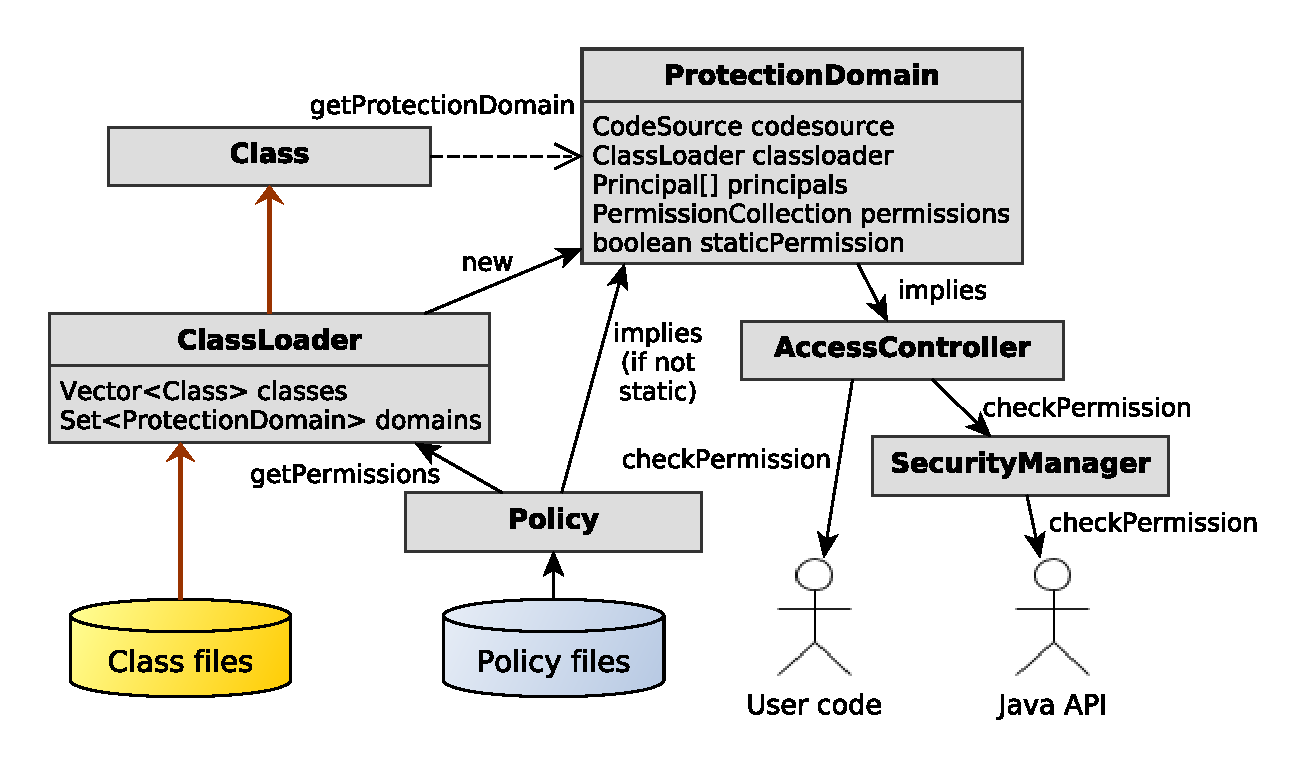
\includegraphics[width=14cm]{fig/domain-schema}
  \caption{Diagram datových toků oprávnění tříd v Javě}
  \label{diagramDatovychToku}
\end{figure}

Diagram datových toků na obrázku \ref{diagramDatovychToku} ukazuje putování informace o oprávněních třídy ze souboru bezpečnostní politiky až k systému řízení přístupu a správci bezpečnosti. Souvislé černé šipky představují přenos informace o oprávněních, zatímco hnědé o třídách. Přerušované šipky představují reference. Směr šipky pak vede z třídy objektu s referenční proměnnou do třídy referencovaného objektu.

Ochranné domény a tím i statická oprávnění třídy jsou třídám přidělovány při jejich zavádění. Objekty ochranných domén ({\tt ProtectionDomain}) vytváří zavaděč tříd a to na základě jejich zdroje kódu ({\tt CodeSource}). Na statická oprávnění, která má zdroji kódu (a tedy i vytvořené ochranné doméně) zavaděč přidělit, se dotazuje aktuálně používaného objektu bezpečnostní politiky ({\tt Policy}).

Výstupem zavaděče tříd pak je objekt třídy ({\tt java.lang.Class}), jež nese referenci na svoji ochrannou doménu, která je společná všem objektům se stejným zdrojem kódu.

Systém řízení přístupu ({\tt java.security.AccessController}) pak rozhoduje na základě oprávnění v ochranné doméně a není-li ochranná doména označena jako používající výhradě statická oprávnění, také na základě odpovědi objektu bezpečnostní politiky ({\tt Policy}).

Na systém řízení přístupu pak rozhodování deleguje také standardní správce bezpečnosti ({\tt java.lang.SecurityManager}).


%%%%%%%%%%%%%%%%%%%%%%%%%%%%%%%%%%%%%%%%%%%%%%%%%%%%%%%%%%%%%%%%%%%%%%%%%%%%%%
\chapter{Distribuované prostředí Red Hat JBoss}
%%%%%%%%%%%%%%%%%%%%%%%%%%%%%%%%%%%%%%%%%%%%%%%%%%%%%%%%%%%%%%%%%%%%%%%%%%%%%%

WildFly, dříve známý jako JBoss AS, je aplikační server standardu Java EE. Poskytuje tedy běhové prostředí Java EE aplikacím, které se na tento aplikační server nainstalují.

Instalace WildFly je možné spojit do domény a vytvořit tak distribuované prostředí. Každou instalaci WildFly pak nazýváme hostitelem. Doména je tedy skupinou hostitelů ({\tt host}), přičemž na jediném počítači může teoreticky běžet více hostitelů. Typicky však jeden hostitel odpovídá jednomu počítači.

Jeden z hostitelů plní funkci doménového řadiče ({\tt domain controller}). Tento hostitel je nositelem jediného používaného konfiguračního souboru domény, {\tt domain.xml}. Každý z hostitelů je konfigurován svým konfiguračním souborem {\tt host.xml}, jež určuje, zda-li je hostitel doménovým řadičem nebo, v případě že doménovým řadičem není, adresu doménového řadiče, na který by se tento hostitel měl registrovat. \cite{jbossDomainSetup}

Na každém hostiteli může běžet více serverů -- instancí aplikačního serveru běžících ve vlastních JVM. Každý server má vlastní jméno, jímž se registruje v doméně, sadu portů na kterých poskytuje své služby a JVM ve které běží. Vše z uvedeného je přitom součástí definice serveru v konfiguračním souboru hostitele, {\tt host.xml}. \cite{jbossDomainSetup}

Server je také zařazen do jedné ze skupin serverů, jež jsou definovány v konfiguračním souboru domény. Přiřazení serveru do skupiny je součástí definice serveru v konfiguračním souboru hostitele. \cite{jbossDomainSetup}

Skupiny serverů tedy seskupují servery napříč hostiteli s některými společnými vlastnostmi -- aplikace (deployment) je typicky nasazována na celou skupinu serverů najednou a konfigurace skupiny umožňuje provést nastavení (např. nastavit parametr JVM) na všech serverech skupiny najednou. \cite{jbossDomainSetup}

%=============================================================================
\section{Běh WildFly pod Java Security Managerem}
%=============================================================================

Nakonfigurovat použití Správce bezpečnosti na aplikačním serveru WildFly je možné stejně jako na jekékoli jiné aplikaci v Javě -- nastavením patřičných konfiguračních vlastností popsaných v kapitolách \ref{souborPolitiky} a \ref{securityManager} při startu JVM. To je nejjednodušeji možné zajistit parametrem {\tt -D} příkazu {\tt java}. Ve spouštěcím skriptu WildFly ({\tt standalone.sh} / {\tt domain.sh} / {\tt standalone.bat} / {\tt domain.bat}) je pro tyto potřeby používána proměnná {\tt JAVA\_OPTS}. Připojením parametrů na konec této proměnné tak dosáhneme nastavení použití security manageru a bezpečnostní politiky ve všech JVM aplikačního serveru: \cite{jbossSecurityManager}

\begin{verbatim}
JAVA_OPTS="$JAVA_OPTS -Djava.security.manager"
JAVA_OPTS="$JAVA_OPTS -Djava.security.policy==directory/wildfly.policy"
\end{verbatim}

Jestliže budeme dále předpokládat, že cílem nasazení bezpečnostních politik na server je omezení možností uživatelských aplikací, můžeme od jemného přidělování jen nejnezbytnějších oprávnění součástem WildFly které je nezbytně potřebují, ustoupit k přidělení všech oprávnění všem součástem aplikačního serveru. Uživatelské aplikace nyní ponecháme bez jakýchkoli oprávnění a vyzkoušíme účinky této bezpečnostní politiky:

\begin{verbatim}
grant codeBase "file:${jboss.home.dir}/jboss-modules.jar" {
    permission java.security.AllPermission;
};
grant codeBase "file:${jboss.home.dir}/modules/-" {
    permission java.security.AllPermission;
};
\end{verbatim}

S použitím této bezpečnostní politiky se server WildFly skutečně bez potíží spustí. Když však na tento server nasadíme aplikaci provádějící kupříkladu čtení souboru uloženého v adresáři této aplikace, zjistíme že aplikace nemá problém tento soubor číst. Do souboru ležícího mimo jeho adresář se ale naopak nedostane dokonce ani pokud toto oprávnění benevolentně přidělíme všem programům v JVM bez ohledu na jejich kořen balíčků ({\tt codeBase}).

Protože, použijeme-li naopak prázdný soubor bezpečnostní politiky, start serveru se nezdaří, je očividné že bezpečnostní politika byla nastavena správným způsobem, ale po startu aplikačního serveru byla aplikačním serverem ignorována.

Krokováním programu jsem našel dvě překážky, jež způsobovaly neúčinost bezpečnostní politiky ze souboru bezpečnostní politiky. Obě popisují následující kapitoly.

%=============================================================================
\section{Security manager WildFly}
%=============================================================================

První překážka byla nalezena ve správci bezpečnosti WildFly -- správci bezpečnosti používaném ve WildFly za účelem maximální optimalizace rychlosti aplikačního serveru.

Správce bezpečnosti WildFly používá vláknově lokální proměnnou {\tt CHECKING} pro omezení působnosti správce bezpečnosti. Je-li hodnota této proměnné referencí na objekt {\tt Boolean.TRUE}, jsou bezpečnostní kontroly akcí kontrolovaných správcem bezpečnosti prováděny. Jinak prováděny nejsou a kód pak běží stejně jako by správce bezpečnosti nebyl použit. \cite{sourceWildFlySecurityManager} (Dále v této kapitole bude používáno vyjádření, že správce bezpečnosti běží se zapnutými nebo s vypnutými kontrolami.)

Všechna vlákna WildFly pak implicitně běží se správcem bezpečnosti s vypnutými kontrolami. Kontroly by měly být zapnuty před zahájením provádění uživatelského kódu a opět vypnuty po jeho opuštění. \cite{sourceWildFlySecurityManager}

Toto je zvně správce bezpečnosti WildFly možné provést za pomoci metody {\tt WildFlySecurityManager.doChecked()}, jež zapne bezpečnostní kontroly správce bezpečnosti, provede kód jež jí je předán a následně bezpečnostní kontroly opět vypne. Zapnutí i vypnutí kontrol je přitom přeskočeno, byly-li už kontroly v době volání metody zapnuté, čímž je předejito problémům při vnořeném volání této metody. \cite{sourceWildFlySecurityManager}

Problémem však byla absence použití této metody při volání uživatelského kódu vyřizujícího HTTP požadavky. Tento problém jsem vzhledem k jeho rozsahu dočasně, pro potřeby řešení této práce, vyřešil vytvořením záplaty:

\begin{lstlisting}[caption=Záplata správce bezpečnosti WildFly nastavující bezpečnostní kontroly na implicitně zapnuté, label=patchSM]
-    private static final InheritableThreadLocal<Boolean> CHECKING
                 = new InheritableThreadLocal<>();
+    private static final InheritableThreadLocal<Boolean> CHECKING
                 = new InheritableThreadLocal<Boolean>(){
+        protected Boolean initialValue(){
+            return TRUE;
+        }
+    };
\end{lstlisting}

Tato záplata zajišťuje inicializaci proměnné {\tt CHECKING} na hodnotu {\tt TRUE}. Tato proměnná je vláknově lokální, každé vlákno má tedy její hodnotu uloženou zvlášť, přestože se jedná o vlastnost jednoho objektu. Navíc je tato vláknově lokální proměnná dědičná -- to znamená, že při vytvoření nového vlákna dědí toto vlákno hodnotu této proměnné svého rodičovského vlákna. \cite{refInheritableThreadLocal}\cite{refThreadLocal}

Hodnota proměnné je inicializována při prvním pokusu o získání její hodnoty metodou {\tt get()}, nebyla-li dříve nastavena voláním metody {\tt set()}. Hodnota na kterou je proměnná incializována je určena voláním metody svého objektu, {\tt initialValue()}. Tato metoda vrací implicitně {\tt null}. Jiné implicitní hodnoty lze dosáhnout přepsáním této metody vlastní implementací. Právě přepisem této metody je stanovena i implicitní hodnota proměnné {\tt CHECKING} v mé záplatě na {\tt TRUE} (Kód \ref{patchSM}). \cite{refThreadLocal}

Tato záplata ale zapíná bezpečnostní kontroly pro celou JVM -- popírá tak původní smysl správce bezpečnosti Wildfly, kterým měla být maximální rychlostní optimalizace aplikačního serveru, na což jsem byl také upozorněn při žádosti o začlenění mé záplaty do vývojové verze WildFly Security Manageru jeho vývojáři. \cite{smPullRequest}

Pravděpodobně protože hledání trvalého a koncepčního řešení trvalo již skoro půl roku, byla nakonec, i přes její nekoncepčnost, mnou navržená změna začleněna. \cite{smPullRequest}\cite{smPullRequestImpl}

Další změnou provedenou ve správci bezpečnosti WildFly pro potřeby řešení této práce bylo povolení změny správce bezpečnosti. Tato změna byla nezbytná pro vypínání správce bezpečnosti ze subsystému navrhovaného a popsaného v následujících kapitolách.

\begin{lstlisting}[caption=Záplata správce bezpečnosti WildFly umožňující vypnutí správce bezpečnosti (zkráceno), label=patchSM]
     public void checkPermission(Permission perm, AccessControlContext context) {
         if (perm.implies(SECURITY_MANAGER_PERMISSION)) {
-            throw access.secMgrChange();
+            //throw access.secMgrChange();
         }
\end{lstlisting}

Jak je vidět, spočívá v prostém zakomentování tohoto omezení v metodě správce bezpečnosti ověřujícího povolení prováděné operace -- {\tt checkPermission()}. Toto omezení sice posiluje bezpečnost systému, avšak oslabuje schopnosti bezpečnostních politik, které tak ztrácí možnost povolit uživatelskému kódu (nebo i kódu modulů WildFly) změnu správce bezpečnosti.

Posílení bezpečnosti navíc není až tak výrazné, považujeme-li kód modulů WildFly za důvěryhodný -- uživatelskému kódu ve výměně správce bezpečnosti nadále brání samotná bezpečnostní politika, není-li její součástí výslovné povolení změny správce bezpečnosti.

%=============================================================================
\section{Zavaděč tříd modulů WildFly}
%=============================================================================

Překonání v předchozí kapitole popsaných problémů se správcem bezpečnosti WildFly však problém neúčinosti souborů bezpečnostní politiky nevyřešilo.

Krokováním programu se mi podařilo zjistit, že oprávnění přidělená v souboru bezpečnostní politiky úspěšně opouští objekt bezpečnostní politiky {\tt sun.security.provider.PolicyFile}, na něj delegující objekt {\tt org.jboss.modules.ModulesPolicy} i na tento objekt delegující objekt {\tt org.jboss.security.jacc.DelegatingPolicy}.

Krokováním programu z opačné strany problému se mi zároveň podařilo zjistit, že v objektu ochranné domény třídy se naopak toto oprávnění nenachází. K zahození oprávnění ze souboru bezpečnostní politiky tedy muselo dojít mezi získáním oprávnění z objektu bezpečnostní politiky a jejich uložením do objektu ochranné domény.

Na základě informací uvedených v kapitole \ref{classloader} jsem tedy zdroj problému dále hledal v zavaděči tříd. Právě on totiž oprávnění z objektu bezpečnostní politiky získává a objekty ochranných domén přitom vytváří a třídám přiděluje.

Zavádění tříd systémových i uživatelských modulů WildFly obstarává Zavaděč tříd modulů ({\tt org.jboss.modules.ModuleClassLoader}). Díky zdrojovému kódu metody {\tt getProtectionDomain()} této třídy se nakonec skutečně podařilo odhalit příčinu ignorování souboru bezpečnostní politiky.

Tato metoda zajišťuje vytvoření objektu ochranné domény a oprávnění, která této doméně přidějí, získává ze dvou zdrojů. Prvním zdrojem ({\tt permissions}) jsou oprávnění modulu aplikačního serveru, definovaná konfiguračním souborem {\tt permission.xml} v archivu modulu. Účel i forma tohoto konfiguračního souboru jsou určeny specifikací Java EE. \cite{javaEEspec} Druhým zdrojem ({\tt policyPermissions}) pak jsou oprávnění získaná z objektu bezpečnostní politiky.

Metoda standardně přiděluje ochranným doménám oprávnění pouze z jejich modulů a oprávnění z objektu bezpečnostní politiky ignoruje. Jak se však ze zdrojového kódu tohoto zavaděče podařilo zjistit, používaná množina oprávnění může být také sjednocením oprávnění z objektu bezpečnostní politiky a oprávnění modulu.

Toho je možné dosáhnout nastavením konfigurační vlastnosti {\tt jboss.modules.policy-permissions} na {\tt true}. Hlavním problémem tak byla absence dokumentace ke způsobu vynucení použití souborů bezpečnostní politiky v prostředí WildFly.

\begin{lstlisting}[caption=Způsob nastavení spuštění aplikačního serveru se souborem bezpečnostní politiky, label=jbossOpts]
JAVA_OPTS="$JAVA_OPTS -Djboss.modules.policy-permissions=true"
JAVA_OPTS="$JAVA_OPTS -Djava.security.manager"
JAVA_OPTS="$JAVA_OPTS -Djava.security.policy==directory/wildfly.policy"
\end{lstlisting}

Výsledný výčet příkazů, jejichž přidáním do startovacího skriptu (např. {\it standalone.sh}) zajistíme spuštění aplikačního serveru se souborem bezpečnostní politiky, ukazuje Kód \ref{jbossOpts}.

Konfigurační proměnná {\tt java.security.manager} zajistí použití správce bezpečnosti a {\tt java.security.policy} stanoví soubor bezpečnostní politiky používaný implicitní implementací třídy bezpečnostní politiky, jak již bylo popsáno v kapitole \ref{souborPolitiky}.

Samotná proměnná {\tt jboss.modules.policy-permissions} nastavena na {\tt true} pak v prostředí aplikačního serveru WildFly zajistí, že budou oprávnění stanovená objektem bezpečnostní politiky používána.

%%%%%%%%%%%%%%%%%%%%%%%%%%%%%%%%%%%%%%%%%%%%%%%%%%%%%%%%%%%%%%%%%%%%%%%%%%%%%%
\chapter{Návrh systému}
%%%%%%%%%%%%%%%%%%%%%%%%%%%%%%%%%%%%%%%%%%%%%%%%%%%%%%%%%%%%%%%%%%%%%%%%%%%%%%

Cílem práce je vytvoření systému pro centralizovanou správu a distribuci bezpečnostních politik. Měl by umožnit nasazovat bezpečnostní politiky na jednotlivé servery domény WildFly a sledovat také, které bezpečnostní politiky jsou právě na kterých serverech domény WildFly nasazeny.

Jako příhodné se pro tento účel zdá využití rozšiřitelnosti systému WildFly a implementace zmíněné funkcionality formou subsystému aplikačního serveru WildFly. Subsystém je rozšířením aplikačního serveru a jeho konfigurace i přítomnost je nastavována zvlášť pro každý profil, přičemž profil je souhrnem konfigurace serveru a je nastavovaný pro celé skupiny serverů. Optimálním řešením by bylo takové rozšíření WildFly, jež by bylo nasazováno a konfigurováno nezávisle na profilech jednotlivých serverů. Takový koncept ale bohužel WildFly neposkytuje.

Nadále proto budeme předpokládat, že všechny skupiny serverů, v rámci kterých chceme s bezpečnostními politikami manipulovat, používají stejný konfigurační profil.

%=============================================================================
\section{Způsob nastavení bezpečnostní politiky}
%=============================================================================

Uživatel i aplikace mohou se subsystémem komunikovat prostřednictvím JBoss native management API. To je navrženo pro maximální jednoduchost a k nejrůznějším nastavením, které by jinak byly reprezentovány objekty velkého množství tříd, je možné přistupovat jako ke stromu objektů obecných tříd uzel ({\tt ModelNode}) a vlastnost (Property). Uzly tvoří strom a každý uzel může mít vlastnosti, jež obsahují samotnou konfiguraci aplikačního serveru ve formě textových řetězců ({\tt String}), do kterých tedy musí být převedeny i hodnoty jiných datových typů. \cite{jbossDetypedManagement}

Klient JBoss native management API, kterým jsou zejména CLI rozhraní WildFly a Webová konzola WildFly, tedy musí implementovat jen práci s tímto konfiguračním stromem. Jeho implementace tedy teoreticky nemusí vůbec záviset na typu informace v konfiguračním stromu. V praxi toto ale pochopitelně platí jen pro nízkoúrovňové nástroje sloužící k přímé úpravě konfiguračního stromu, jakým je CLI rozhraní WildFly. Webová konzola naproti tomu pracuje s více konkrétními třídami objektů, jakými jsou server, skupina ({\tt server-group}) nebo zdroj dat ({\tt datasource}). Přestože pracuje se stejným konfiguračním stromem, tvořeným jen těmito dvěma datovými typy, je závislá na struktuře kterou uzly tohoto stromu tvoří. Jednoduchost JBoss native management API je tak znatelná spíše jen na stabilitě tohoto API a knihovně pro práci s ním -- {\tt jboss-dmr}. \cite{jbossDetypedManagement}

Rozšíření aplikačního serveru, kterým je například subsystém, vykonává svůj kód zejména v reakci na události, které si zaregistruje. Těmito událostmi bývá zpravidla načtení rozšíření a přidání a odebrání subsystému, často také operace nad uživatelským balíčkem (nasazení apod.) nebo právě operace nad definovanou konfigurační vlastností. \cite{WildFlyExtending}

Jako vhodné řešení bylo tedy zvoleno nasazení bezpečnostní politiky v návaznosti na nastavení hodnoty konfigurační proměnné. Každý server aplikačního serveru bude mít v konfiguračním stromu svůj uzel a jeho vlastnostmi bude bude určen soubor bezpečnostní politiky, jež by měl být nasazený na daném serveru a také to, zda by měl být security manager pro daný server vůbec zapnutý.

Samotná operace provedení výměny bezpečnostní politiky a případného zapnutí/vypnutí security manageru pak bude spojena s událostí nastavení hodnoty dané vlastnosti. Vlastnosti bude přiřazena metoda, jež má být volána při zápisu do její hodnoty. Ta zajistí výměnu bezpečnostní politiky prostřednictvím k tomu určené třídy, jež bude součástí vytvářeného subsystému.

%=============================================================================
\section{Způsob šíření souborů bezpečnostní politiky} \label{sireniSouboru}
%=============================================================================

Jelikož cílem práce není jen centralizovaná správa, ale i distribuce bezpečnostních politik, je nutné rovněž stanovit způsob, jakým soubory bezpečnostní politiky budou šířeny mezi servery WildFly domény.

Jako pravděpodobně nejjednodušší řešení, které by bylo možné navrhnout, lze označit vytvoření sdíleného adresáře, jež by byl přístupný z každého serveru domény, například protokolem NFS (Network File System).

S tímto řešením však souvisí hned několik potíží. První z nich je vyšší platformní závislost -- zatímco WildFly jakožto aplikace v Javě bez problému běží na mnoha platformách a pod různými operačními systémy, protokol NFS není napříč operačními systémy příliš podporován. Tento problém by bylo možné řešit použitím více rozšířeného protokolu umožňujícího vzdálený přístup k souborům, jakým je například FTP.

Druhým problém je ale bezpečnost -- protokoly FTP ani NFS samy o sobě nedokáží zaručit autenticitu serveru, ke kterému se klient připojuje. Případný útočník by se tak mohl vydávat za FTP/NFS server na němž jsou bezpečnostní politiky uložené a podvrhnout tak serverům domény vlastní bezpečnostní politiky. Tento problém by mohlo vyřešit použití lépe zabezpečeného protokolu, jakým je například SSH (Secure Shell), jež umožňuje vzdálený přístup k souborům prostřednictvím SSHFS (SSH Filesystem), nebo FTPS (FTP over SSL), kde se server vůči klientovi autentizuje za pomoci asymetrické kryptografie. \cite[3]{ssh}

Použití těchto lépe zabezpečených protokolů zajistí bezpečnost systému, avšak umocní problém platformních omezení, obzvláště v případě protokolu SSH. Navíc i v případě dokonalého zajištění sdíleného adresáře bezpečnostních politik bude nutné zajistit také bezpečný přenos informací po JBoss Native API, pro bezpečný přenos informace, kterou bezpečnostní politiku má daný server použít.

Problém bezpečnosti distribuce bezpečnostních politik je možné si představit jako řetěz. Řetěz je jen tak silný, jak silný je jeho nejslabší článek. Aby byl řetěz silný, je třeba mít silné všechny jeho články -- v tomto případě bezpečnost komunikačního kanálu, po kterém se přenáší soubory bezpečnostních politik a komunikačního kanálu, po kterém se přenáší informace, který soubor bezpečnostní politiky by měl daný server použít.

Touto úvahou lze dojít k závěru, že optimálním řešením je minimalizovat počet článků řetězu -- sloučit tyto dva komunikační kanály do jediného a nadále řešit bezpečnost jen tohoto jediného komunikačního kanálu.

Toto lze implementovat za pomoci uzlů konfiguračního stromu jednotlivých politik představujících jednotlivé soubory politik. Vlastností tohoto uzlu by pak obsah samotného souboru bezpečnostní politiky. Soubory bezpečnostní politiky by pak mohly být nahrávány do těchto vlastností konfiguračních uzlů na straně doménového řadiče a naopak z nich čteny na straně ostatních členských serverů WildFly domény.

Protože však použití standardní třídy bezpečnostní politiky ({\tt sun.security.provider.PolicyFile}) vyžaduje soubory bezpečnostní politiky přístupné skrze URL adresu souboru, je na straně členských serverů třeba před aplikací bezpečnostní politiky obsah souboru bezpečnostní politiky zapsat do dočasného souboru.

Protože bude tento postup nezbytné aplikovat na straně členských serverů domény, je zbytečné řešit toto na doménovém řadiči jinak. Ztrácí se tak také většina důvodů pro to, aby byly bezpečnostní politiky na straně doménového řadiče uloženy v souboru souborového systému.

Jako výhodnějším řešením se tedy začíná jevit ukládat bezpečnostní politiky přímo do vlastností konfiguračních uzlů. Tím bude vyřešen i problém, jak ze strany aplikačního serveru detekovat, že byl soubor bezpečnostní politiky změněn. Zatímco v případě souboru by bylo nezbytné se periodicky dotazovat na čas poslední změny tohoto souboru, na změnu hodnoty konfigurační vlastnosti je možné navázat programovou událost, a tím zajistit aplikaci bezpečnostní politiky přímo v návaznosti na změnu hodnoty její konfigurační vlastnosti.

%=============================================================================
\section{Webové uživatelské rozhraní} \label{navrhGUI}
%=============================================================================

Součástí zadání práce bylo také vytvořit webové rozhraní pro komunikaci s uživatelem. Jelikož je samotné jádro řešení implementováno jako subsystém WildFly, jako optimální řešení se nabízí implementovat uživatelské rozhraní tohoto subsystému jako rozšíření webové konzoly WildFly.

Webová konzola WildFly je standardní součástí aplikačního serveru WildFly. Je GWT aplikací běžící na straně klienta, ve webovém prohlížeči, a se serverem komunikuje prostřednictvím HTTP Management API. To je alternativou Native API -- plní stejnou funkci, ale běží nad protokolem HTTP. Tělem odpovědí serveru i tělem POST dotazů klienta je JSON reprezentace uzlu konfiguračního stromu ({\tt ModelNode}). \cite{WildFlyManagementAPIreference}

\begin{figure}[ht]
  \centering
  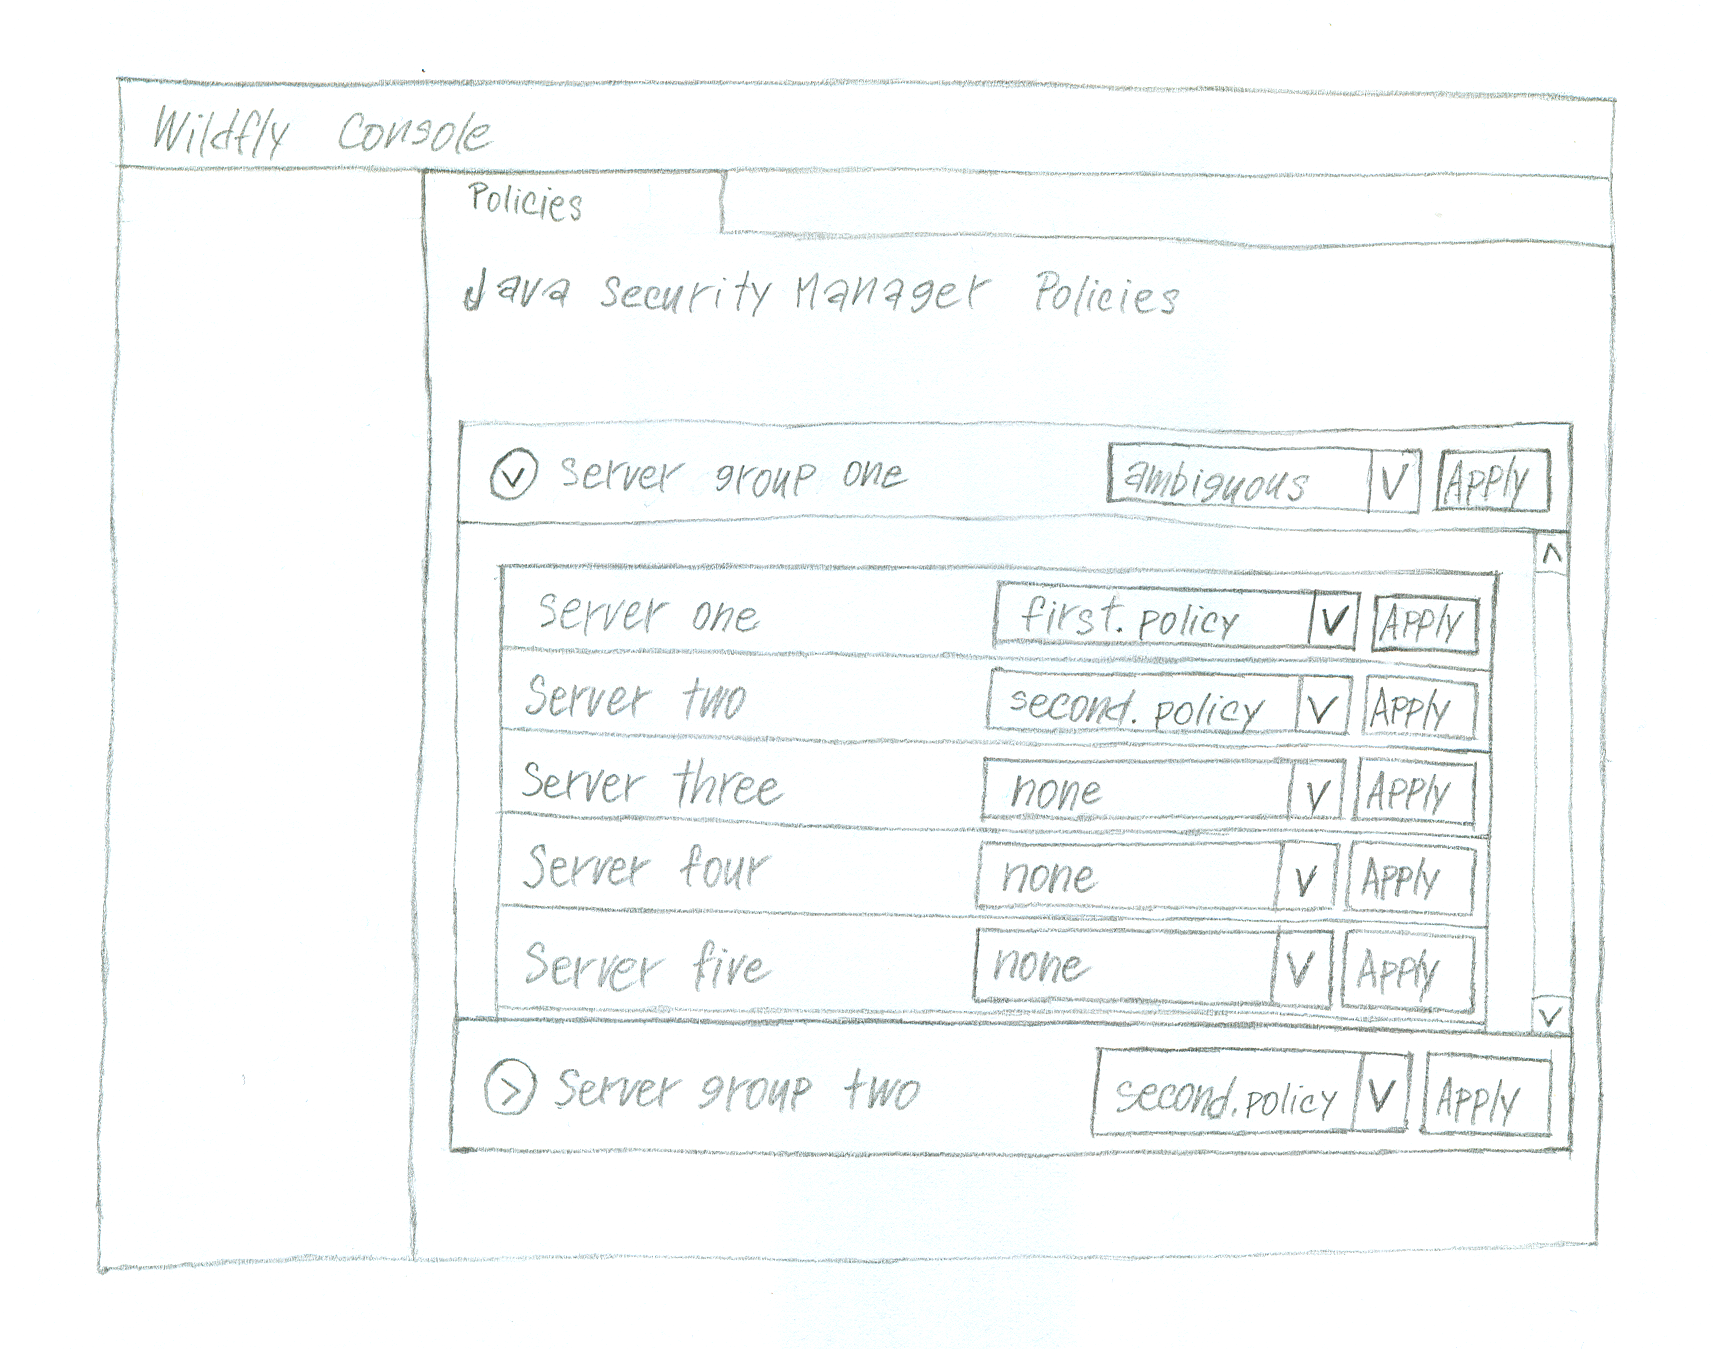
\includegraphics[width=14cm]{fig/mockup}
  \caption{Grafický návrh uživatelského rozhraní plánovaného rozšíření WildFly.}
\end{figure}

%%%%%%%%%%%%%%%%%%%%%%%%%%%%%%%%%%%%%%%%%%%%%%%%%%%%%%%%%%%%%%%%%%%%%%%%%%%%%%
\chapter{Popis implementace systému} \label{implementace}
%%%%%%%%%%%%%%%%%%%%%%%%%%%%%%%%%%%%%%%%%%%%%%%%%%%%%%%%%%%%%%%%%%%%%%%%%%%%%%

%=============================================================================
\section{První etapa}
%=============================================================================

V rámci první etapy implementace řešení byl implementován jednoduchý subsystém WildFly za pomoci kostry subsystému z Maven repozitáře, podle dokumentace WildFly 8 věnující se právě vytváření rozšíření WildFly. \cite{WildFlyExtending}

Dle tohoto vzoru byl vytvořen subsystém, jehož jedinou funkcí bylo rozšíření konfiguračního stromu o uzly {\tt server=*} uchovávající informaci o URL bezpečnostních politik, jež by měly být uloženy na jednotlivých serverech domény WildFly odpovídajících svým jménem jménu tohoto konfiguračního uzlu. Tyto uzly fungovaly jako běžné uzly konfiguračního stromu WildFly -- administrátor měl možnost je vytvářet, odstraňovat a nastavovat jejich vlastnost {\tt policy}, jež nesla právě samotnou URL nasazené bezpečnostní politiky.

Na změnu této konfigurační vlastnosti zároveň server domény daný jménem uzlu reagoval právě nasazením dané bezpečnostní politiky, prostřednicvím registrace této události při tvorbě konfigurační vlastnosti {\tt policy} uzlu {\tt server=*}.

Toho bylo dosaženo vytvořením třídy {\tt ServerWriteAttributeHandler} a jejím uvedením v rámci volání provádějícího registraci samotné konfigurační vlastnosti:

\begin{verbatim}
resourceRegistration.registerReadWriteAttribute(POLICY,
                null, ServerWriteAttributeHandler.INSTANCE);
\end{verbatim}

Není stanovena třída zprostředkovávající čtení tohoto konfigurační vlastnosti. (Na jejím místě je uveden {\tt null}) Na čtení této vlastnosti není totiž vázána žádná akce, ani není nutné obsah vracený jako odpověď na pokus o čtení vlastnosti nikterak upravovat a je možné uživatele nechat číst samotnou vlastnost přímo.

Aby byla bezpečnostní politika aplikována nejen na základě akce administrátora, ale také automaticky po startu serveru, byla její aplikace navázána také na akci přidání nového uzlu {\tt server=*}. Odstranění takového uzlu pak bude navázáno na odebrání bezpečnostní politiky, stejně jako kdyby byla vlastnost {\tt policy} nastavena na nedefinovanou.

Obě akce je jsou implementovány jako třídy {\tt ServerAdd} a {\tt ServerRemove}, jež jsou na uzly typu {\tt server=*} navázány skrze parametry konstruktoru třídy definující tento uzel konfiguračního stromu:

\begin{verbatim}
public class ServerDefinition extends SimpleResourceDefinition {
    private ServerDefinition() {
        super(JsmPolicyExtension.SERVER_PATH,
                JsmPolicyExtension.getResourceDescriptionResolver("server"),
                ServerAdd.INSTANCE,
                ServerRemove.INSTANCE);
    }
}
\end{verbatim}

Konfigurační uzly {\tt server=*} jsou ukládány do konfiguračního XML souboru domény WildFly, jak je u konfigurační uzlů WildFly běžné. Ukládání veškeré konfigurace subsystému je implementováno ve třídě {\tt SubsystemParser}.

%=============================================================================
\section{Druhá etapa}
%=============================================================================

V rámci druhé etapy bylo uživatelské rozhraní pozměněno dle grafického návrhu předvedeného v kapitole \ref{navrhGUI}. V souvislosti s touto změnou bylo nutné rozšířit rovněž subsystém WildFly. Jeho dosavadní implementace neumožňovala výběr bezpečnostní politiky formou výběru v rozbalovací nabídce.

Výběr formou rozbalovací nabídky vyžaduje od aplikace zobrazující nabídku znalost voleb, mezi nimiž může uživatel provádět výběr. To při dosavadní implementaci subsystému možné nebylo, neboť aplikace běžící na straně webového prohlížeče měla přístup k souborům (tedy i souborům bezpečnostních politik) možný jen právě prostřednictvím subsystému, který doposud přístup k seznamu souborů bezpečnostních politik neumožňoval.

Do konfiguračního stromu subsystému tak vedle dosavadních uzlů {\tt server=*} popsaných v minulé podkapitole přibyly uzly {\tt policy=*}, jež reprezentovaly právě jednotlivé soubory bezpečnostní politiky, jež bylo možné jako bezpečnostní politiky jednotlivých serverů nastavit. Tyto uzly nebyly ukládány do konfiguračního XML souboru aplikačního serveru, ale byly vytvářeny ze seznamu souborů nacházejících se v k tomu určeném adresáři aplikačního serveru.

Toto načítání seznamu souborů nebylo řešeno cestou ideální, za kterou by šlo nejspíše považovat přímé navázání jakéhokoli pokusu o čtení těchto konfiguračních uzlů na programovou obsluhu, jež by umožnila jako přímý výsledek tohoto dotazu vrátit přímo aktuální seznam souborů v adresáři bezpečnostních politik.

Vzhledem k ranosti této verze a odstranění těchto schopností systému v pozdějších etapách vývoje bylo načtení seznamu souborů bezpečnostních politik řešeno přímým vytvořením těchto konfiguračních uzlů při startu aplikačního serveru na základě obsahu adresáře bezpečnostních politik ve chvíli startu aplikačního serveru.

Hlavní nevýhodou tohoto přístupu byla přetrvávající potřeba zajištění přístupu k souborům bezpečnostních politik uložených na doménovém řadiči, nikoli však již na jednotlivých aplikačních serverech domény. Adresář bezpečnostních politik tak bylo nutné napříč aplikačními servery distribuovat jinou cestou. (Podrobněji popsanou v kapitole \ref{navrhGUI} zabývající se návrhem právě způsobu šíření souboru bezpečnostních politik.)

Později odhaleným nedostatkem se pak stal fakt, že do konfigurační vlastnosti {\tt policy} byla ukládána absolutní cesta k souboru bezpečnostní politiky, což by výrazně zkomplikovalo ostré nasazení implementovaného systému.

%=============================================================================
\section{Třetí etapa}
%=============================================================================

V rámci třetí etapy implementace byl subsystém WildFly upraven, aby konfigurační strom WildFly nefungoval jen jako úložiště adres nastavených bezpečnostních politik, ale také jako úložiště samotných bezpečnostních politik.

Byl tedy pozměněn význam konfigurační vlastnosti {\tt file} uzlu {\tt policy=*}. Absolutní URL adresa souboru  bezpečnostní politiky byla nahrazena obsahem souboru bezpečnostní politiky.

Zároveň byl změněn význam konfigurační vlastnosti {\tt policy} uzlu {\tt server=*}, jež doposud rovněž obsahoval URL adresu souboru bezpečnostní politiky nasazené na daném serveru. Nově byl nahrazen jménem uzlu {\tt policy=*}, jehož bezpečnostní politika z jeho vlastnosti {\tt file} byla na daný server nově nasazována.

Nadále tak nestačilo provádět aplikaci bezpečnostní politiky při změně atributu {\tt policy} uzlu {\tt server=*}, ale bylo nutné bezpečnostní politiku používanou aplikačním serverem vyměnit rovněž při změně obsahu vlastnosti {\tt file} uzlu {\tt policy=*}.

Toto je řešeno analogicky jako právě v případě akce navázané na změnu vlastnosti uzlu serveru -- vytvořením třídy {\tt PolicyWriteAttributeHandler} a jejím navázáním na vlastnost uzlu bezpečnostní politiky.

%%%%%%%%%%%%%%%%%%%%%%%%%%%%%%%%%%%%%%%%%%%%%%%%%%%%%%%%%%%%%%%%%%%%%%%%%%%%%%
\chapter{Testování systému}
%%%%%%%%%%%%%%%%%%%%%%%%%%%%%%%%%%%%%%%%%%%%%%%%%%%%%%%%%%%%%%%%%%%%%%%%%%%%%%

Protože cílem této bakalářské práce nebylo jen vytvoření systému umožňujícího správu bezpečnostních politik nasazených na jednotlivých serverech distribuovaného systému ale také jeho otestování, tato kapitola se zabývá tvorbou testů, umožňujících otestovat implementované řešení.

Testování je nedílnou součástí vývoje software a je užíváno k odhalení vad software a prokázání, že software dosáhl požadované úrovně kvality v zadaných kritériích. Obvykle se provádí za pomoci automatizovaných programů, takzvaných testů. \cite{ivsTest}

Testy se běžně dělí následovně: \cite{testsTypes}\cite{ivsTest}

\begin{enumerate}
  
  \item {\textbf Jednotkové testy (Unit tests)} testují jednotlivé jednotky systému. Jednotkou je typicky třída programovacího jazyka. Každá jednotka se testuje samostatně, s maximální snahou o izolaci od ostatních součástí systému. Jejich cílem je především ověřit, zda jednotlivé jednotky splňují svoji specifikaci -- dodávají na základě testovacího vstupu odpovídající výstup. Nijak neřeší problémy v komunikaci jednotlivých jednotek mezi sebou nebo se zbytkem systému (v tomto případě aplikačním serverem WildFly). \cite{testsTypes}\cite{ivsTest}
  
  \item {\textbf Systémové testy (System tests)} testují celý systém jako jediný celek a umožňují ověřit zda systém jako celek dokáže plnit svůj účel, pro který byl vytvořen. Testovaný systém ovlivňují a kontrolují zpravidla z jeho vnějšku. \cite{testsTypes}\cite{ivsTest}
  
  \item {\textbf Integrační testy (Integration tests)} jsou mezistupněm mezi jednotkovými a systémovými testy. Jak jejich název napovídá, jejich hlavním účelem je ověřit zda spolu testované jednotky správně spolupracují. \cite{testsTypes}\cite{ivsTest}
  
\end{enumerate}

Protože lze systémové testy někdy chápat také jako zvláštní případ integračních testů, jsou systémové testy někdy mezi integrační testy zahrnovány. \cite{testsUnitVsInteg}

%=============================================================================
\section{Jednotkové testy}
%=============================================================================

Jednotkové testy tedy umožňují testovat jednotlivé jednotky systému a těmito jednotkami, po kterých se systém testuje, jsou typicky třídy programovacího jazyka. Každé třídě programu by v ideálním případě měla být přidělena jedna třída testu, jež by měla ověřit správnost fungování této třídy.

Testované jednotky by měly být testovány ve vzájemné izolaci. Toho se dosahuje buď jejich vhodným návrhem, nebo použitím napodobenin objektů ({\it mock object}) z jiných jednotek, na kterých tato jednotka závisí.

Komplikace jež by mohly ohrozit samotnou výměnu bezpečnostní politiky nebo správce bezpečnosti vyplývají převážně z integrace s aplikačním serverem WildFly. Vytvoření jednotkových testů pro výměnu bezpečnostní politiky a správce bezpečnosti by tedy nebylo příliš užitečné.

Byly však vytvořeny jednotkové testy pro testování podpůrných součástí implementovaného subsystému -- testy syntaktické kontroly souborů bezpečnostní politiky a práce s konfiguračním podstromem DMR subsystému.

%=============================================================================
\section{Integrační testy}
%=============================================================================

Integrační testy testují systém jako celek. Implementovaný systém byl tímto způsobem testován na schopnost plnění základních požadavků daných zadáním této práce -- schopnosti zapnout a vypnout správce bezpečnosti a vyměnit používanou bezpečnostní politiku skrze administrační protokol WildFly.

Byl tedy vytvořen integrační test umožňující otestovat zmíněné schopnosti na běžícím aplikačním serveru WildFly s nainstalovaným subsystémem pro nastavení bezpečnostní politiky, jehož vytvoření je popsáno v kapitole \ref{implementace}.

Tento test se skládá ze dvou částí -- agenta, aplikace nasazované na testovaný server, a manažeru -- testu vytvořeného za pomoci knihovny JUnit, řídícího proces samotného testování.

Agent je Java EE aplikací nabízející své služby skrze rozhraní REST. Službami, jež poskytuje, je zejména otestování schopnosti provést vybranou akci z pozice aplikace nasazené na testovaném serveru. Klient rozhraní REST se tedy k této službě může připojit a požádat o otestování schopnosti provést vybranou operaci. Jako odpověď pak dostane informaci, zda-li se provedení této operace zdařilo, nebo zda bylo zmařeno Access controllerem.

Mimo toho tato služba umožňuje manageru zjistit také některé další informace o aplikačním serveru, zjistitelné ze strany aplikace nasazené na tomto aplikačním serveru, jako je aktuálně používaná třída security manageru, používaná třída bezpečnostní politiky, nebo samotná přítomnost agenta na testovaném aplikačním serveru.

Manager je část systémového testu běžící mimo aplikační server. Sestává z testů založených na knihovně JUnit a pomocných tříd {\tt Domain} a {\tt Server}.

Třída {\tt Server} zajišťuje komunikaci manageru s agentem nasazeným na testovaném serveru WildFly prostřednictvím protokolu REST. Některé testy, například testy vzájemného ovlivňování serverů mezi sebou, mohou vyžadovat monitoring více serverů WildFly najednou. Na každém z nich pak musí být nasazena aplikace agenta a s každým z nich pak bude moci test komunikovat prostřednictvím samostatné instance třídy {\tt Server}.

Třída {\tt Domain} mezitím zajišťuje komunikace se samotnou doménou aplikačních serverů prostřednictvím protokolu JBoss Native API. Umožňuje manipulovat s konfiguračním stromem WildFly, zejména přidávat a upravovat hodnoty konfiguračních vlastností uzlů {\tt server=*} a {\tt policy=*} a tím nasazovat bezpečnostní politiky na jednotlivé servery WildFly domény.

Určitý problém, jež bylo nutno vyřešit, zde představuje způsob, jakým po skončení každého testu navrátit systém do původního stavu. Jelikož se jedná o testování z vně aplikačního serveru, není pro tento účel možné využít operaci {\tt rollback}, jež se běžně automaticky provádí při selhání objektu ošetřujícího událost úpravy konfiguračního uzlu.

Budeme-li však předpokládat že testy budou prováděny na k tomu určené doméně aplikačních serverů, můžeme pominout požadavek na navrácení původní konfigurace po ukončení testování a omezit navrácení do původního stavu na navrácení do stavu s prázdným konfiguračním uzlem subsystému, tedy bez jakýchkoli konfiguračních uzlů 
{\tt server=*} nebo {\tt policy=*}.

Další operací objektu domény tak bude navrácení subsystému do počátečního stavu. Toho bude dosaženo spojením operace odstranění uzlu subsystému {\tt jsmpolicy} konfiguračního stromu a jeho opětovné přidání.

%%%%%%%%%%%%%%%%%%%%%%%%%%%%%%%%%%%%%%%%%%%%%%%%%%%%%%%%%%%%%%%%%%%%%%%%%%%%%%
\chapter{Závěr}
%%%%%%%%%%%%%%%%%%%%%%%%%%%%%%%%%%%%%%%%%%%%%%%%%%%%%%%%%%%%%%%%%%%%%%%%%%%%%%

Cílem práce bylo navrhnout, vytvořit a otestovat systém pro centralizovanou správu a distribuci bezpečnostních politik Javy v distribuovaném prostředí aplikačního serveru WildFly.


